% The "%" character denotes a comment
% This file was written by Nathan Moore, Winona State University
% as a template for how lab reports might be written in LaTeX.
% style choices originally come from the American Journal of Physics's
% sample submission file, http://ajp.dickinson.edu/Contributors/manFormat.html
%
%
\documentclass[prb,preprint]{revtex4-1}
\usepackage{amsmath}  % needed for \tfrac, \bmatrix, etc.
\usepackage{amsfonts} % needed for bold Greek, Fraktur, and blackboard bold
\usepackage{graphicx} % needed for figures

%these are some macros (shortcuts)
\newcommand{\bea}{\begin{eqnarray}}
\newcommand{\eea}{\end{eqnarray}}
\newcommand{\be}{\begin{equation}}
\newcommand{\ee}{\end{equation}}

\begin{document}

\title{Microcontrollers Lab 01: PWM and LEDs}
\author{Adam Stammer}
%\email{adam.stammer@go.winona.edu}

\date{\today}

%if you include an abstract, it goes here
\begin{abstract}
Pulse Width Modulation (PWM) is not only a very common tool in digital electronics, but can also serve as a good teaching tool in the programming of microcontrollers. It motivates many of the basics of microcontroller programming like for loops, boolean logic, delays, pin I/O, etc. In this lab we explore various led animations using many of these tools.
\end{abstract}

\maketitle


%These are my general reccomendations for an undergraduate lab report in Physics. 
%
%\textbf{Purpose}
%The lab report should start with a purpose statement.  Briefly 
%provide the necessary background and explain what problem your are trying to 
%solve/investigate.
%
%\textbf{Conclusions} Don't be coy, cut to the point right away and state what you found. This should be breif.
%
%\textbf{Theory} We never just measure stuff in Physics.  There's always a 
%theoretical idea behind the measurement we're making.  Explain  the ideas 
%behind your work, starting at the level of a successful Physics 221/222 
%student.
%
%\textbf{Data} Sketch out, in words and pictures, the apparatus you used to take data.  Report the data, graphically, if possible, and state the uncertainties  in your measurement.  Don't provide pages of computer printout here. Data tables shouldn't be your first choice when it comes to communicating your measurements.\cite{Tufte}
%
%\textbf{Analysis} With data presented, describe how the theory agrees/disagrees with 
%the data you took.  Normally this is accomplished with a fit line (or math 
%model) that is interpreted.
%
%\textbf{Limitations and Recommendations} Every measurement has limitations and it is only honest to report them to the reader.  ``Human Error'' is a meaningless statement.  After your analysis is complete, revisit the purpose statement.  This is the place to more forcefully argue your conclusions.    
%
%Notes: 
%Writing in the first person, eg ``I" or ``We," is fine.
%
%\newpage
%\textbf{Example Lab Report:}

\section{Collecting Data}
The circuit from which data was collected can be seen below, where $R_{p}$ is varied, $R_{LED}$ represents a red Light Emitting Diode (LED), and $V_{cc}=5 Volts$. 

\begin{figure}[ht]
	\centering
	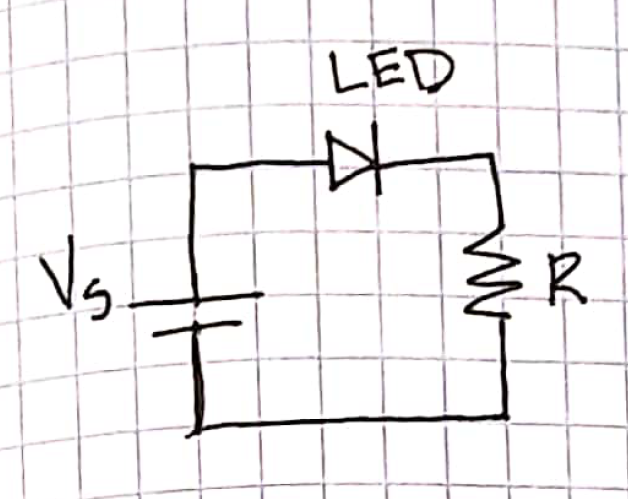
\includegraphics[width=2.5in]{figure1.png}
	\caption{Simplified Circuit Used to Collect Data (Lab 01)}
	\label{fig1}
\end{figure}

First I set up a single LED in series with a resistor to verify it worked. After that I swapped out resistors, measuring the current each time. The collected data can be seen graphed below.

\begin{figure}[ht]
	\centering
	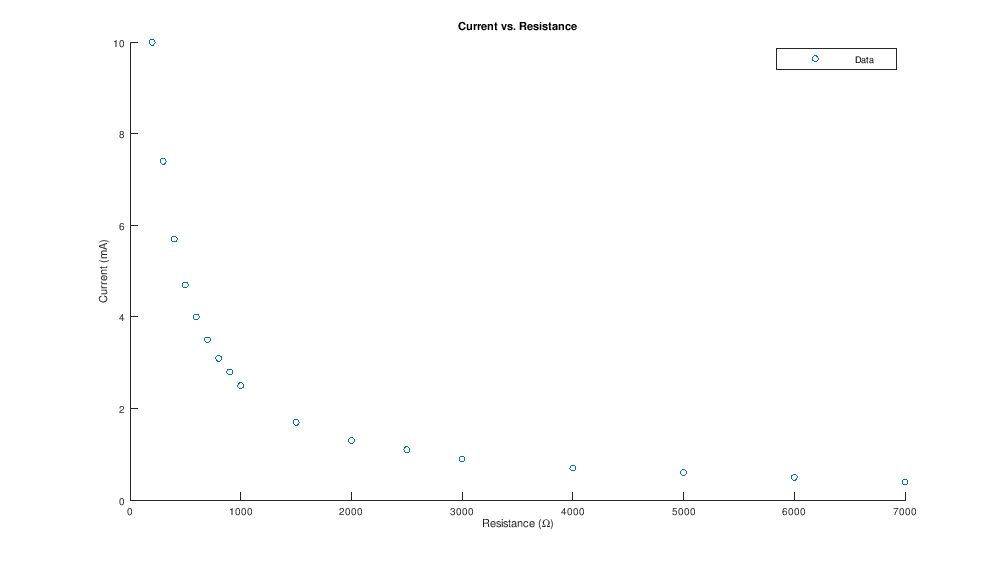
\includegraphics[width=6in]{bigGraph.png}
	\caption{Data Collected}
	\label{fig1}
\end{figure}


Ohm's Laws tells us that the relationship between I and R is linear, such that graphing the two against each other should get us an inverse relationship slope. Which we can indeed see within the graph above.

To linearalize the relationship of this graph we can simply invert the denominator of the relationship. With Ohms Law we can see this relationship should be linear. 

\begin{equation}
V=I\frac{1}{R}
\end{equation}

We do indeed see this relationship in the following graph.

\begin{figure}[ht]
	\centering
	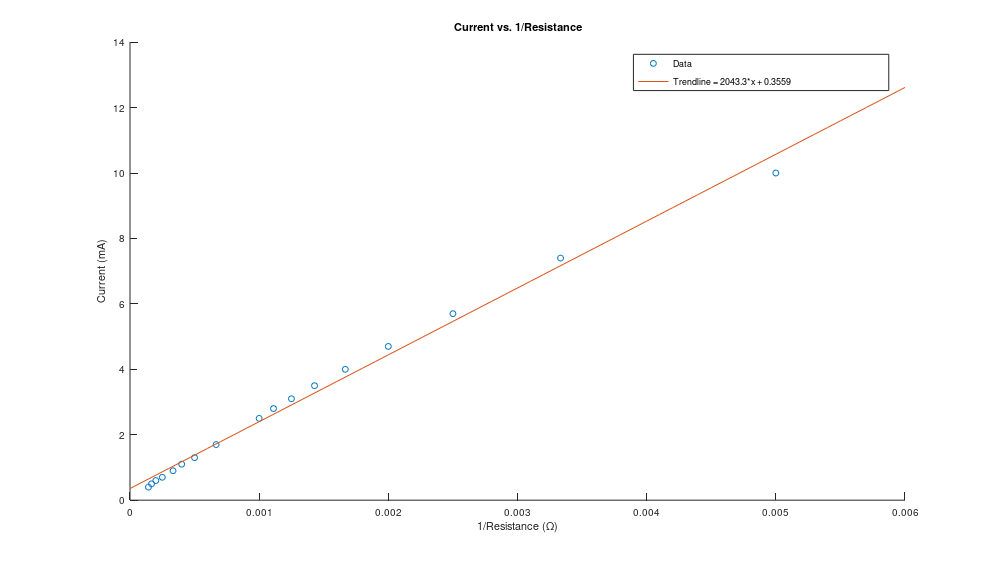
\includegraphics[width=6in]{bigGraph2.png}
	\caption{Data Collected Linearalized}
	\label{fig1}
\end{figure}


\section{Photoresistor}

Next I modified the above circuit to include, in series, a Photoresistor along with the regular resistor. The Photoresistor changes resistance based on how much light is hitting the top of it. The regular resistor was left in the circuit to make sure that the circuit would maintain enough resistance to not fry the arduino pins. You can see this circuit in action at the following link: \url{https://mediaspace.minnstate.edu/media/Micro_Lab01_photoresist/1_brvv6kld}

All code available at the end of this report.

\section{SOS LED}

Using for loops that varied the delay between led flashes I then set an led to blink out an SOS Morse code message. The for loops greatly simplified the varying degrees of delay necessary to flash such a message, although this code is not very easily expandable for more complex messages. This project can be seen in action at the following link: \url{https://mediaspace.minnstate.edu/media/Micro_Lab01_sos/1_24rqkk3p}


All code available at the end of this report.

\section{Breathing LED}
Using PWM we can vary the brightness of our LEDs directly. Turning an LED on for 50 milliseconds, off for 50 milliseconds, and repeat, results in what looks like an LED that is only at half brightness. These delays can be changed such that an LED can be any brightness within a given range. This also can be used to decrease the power consumption of devices like these LEDs. To demonstrate this I then made a 'breathing' LED that has a brightness that grows and then fades, over and over. This project can be seen in action at the following link: \url{https://mediaspace.minnstate.edu/media/Micro_Lab01_breathe/1_09uji2tb}

All code available at the end of this report.


\section{Oscillating Night Rider LEDs}
At this point it seemed appropriate to control multiple LEDs at the same time. To start off with I just stuck with max brightness to keep it simple and make it easier to debug. A for loop going through an array of the output pins was able to achieve this pattern. You can see the circuit drawn below.

\begin{figure}[ht]
	\centering
	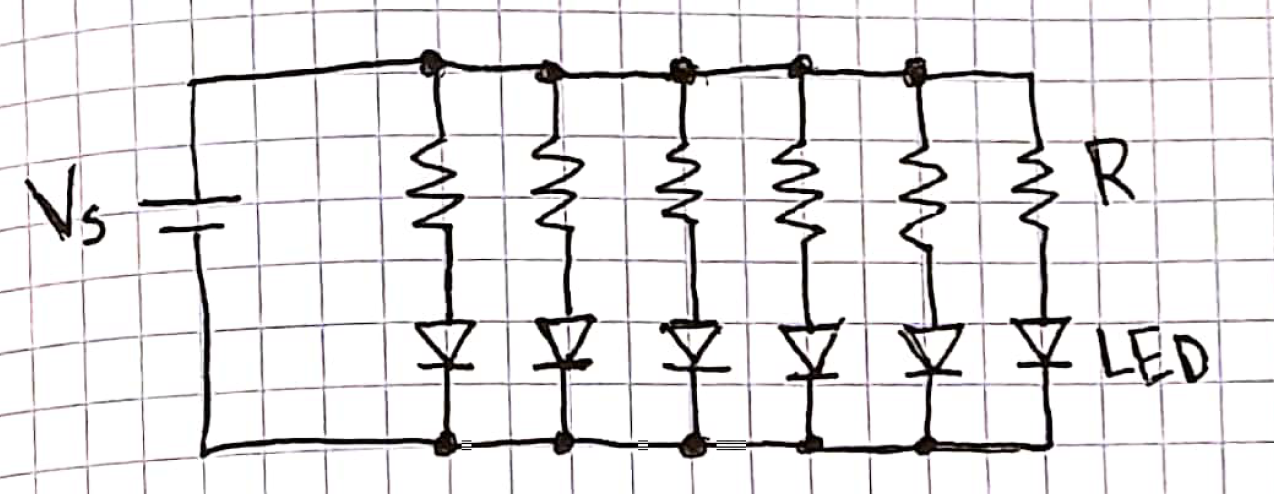
\includegraphics[width=3in]{figure2.png}
	\caption{Multi-LED Circuit Simplified}
	\label{fig1}
\end{figure}

\begin{figure}[ht]
	\centering
	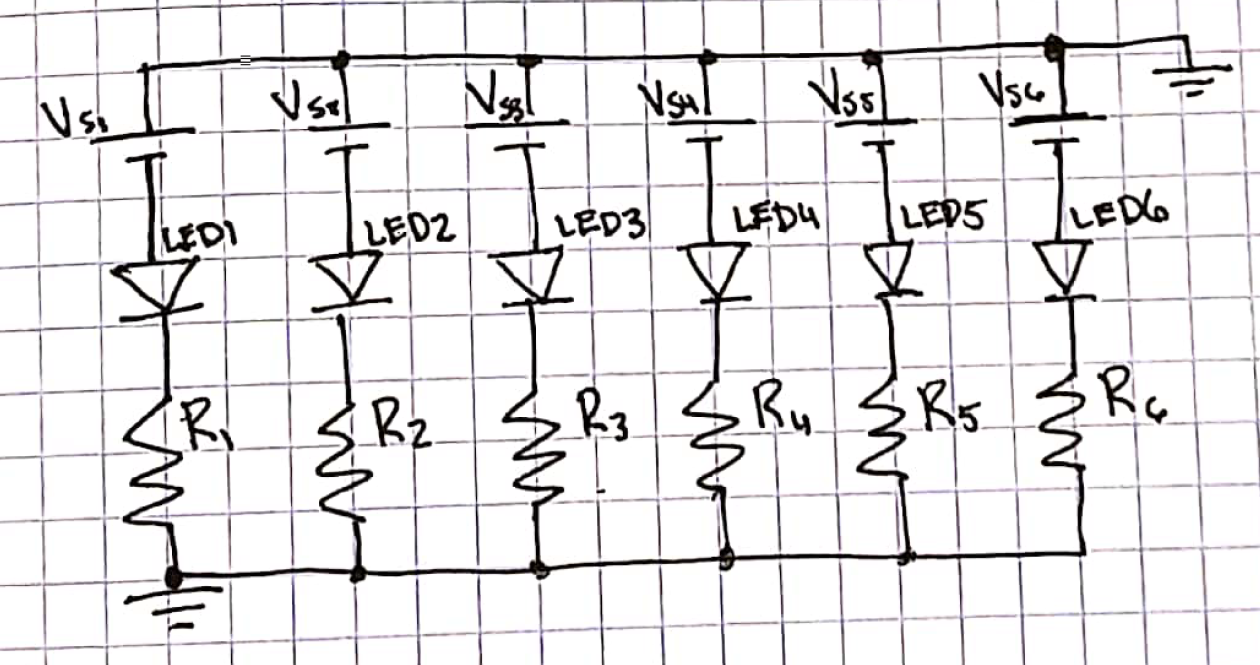
\includegraphics[width=3in]{figure3.png}
	\caption{Multi-LED Circuit}
	\label{fig1}
\end{figure}

This project can be seen in action at the following link: \url{https://mediaspace.minnstate.edu/media/Micro_Lab01_nightrider/1_lwnp2zr1}

All code available at the end of this report.

\section{Fireworks}
To put all of these tools together I then built a multi-led animation meant to mimic fireworks. A central led would light up really bright with neighboring LEDs lighting up dimmer. Then as the animation updates, the bright spot ripples out the neighboring LEDs as the previous ones begin to dim. This was achieved by using multiple for loops to update the static animation itself that was represented as an array of a brightness overlay. For example [0, 2, 4, 2, 0], would represent a 5 LED matrix with the central LED at max brightness, the direct neighboring LEDs at half brightness and their respective neighbors off. This made the animation easy to tweak as each update just requires a new array of respective brightnesses. However to randomly this animation on a 'central node' LED required additional looping and checks to make sure that the updating animation is pushing a brightness to a pin that actually exists. Sometimes the animation would start near the edge of the LED line, so it was important to make sure the LED in question actually exists, and if not to not push any animation to it. The circuit used was the same as that seen above. This project can be seen in action at the following link: \url{https://mediaspace.minnstate.edu/media/Micro_Lab01_fireworks/1_85dmt45w}

All code available at the end of this report.

%\begin{thebibliography}{99}
% The numeral (here 99) in curly braces is nominally the number of entries in
% the bibliography. It's supposed to affect the amount of space around the
% numerical labels, so only the number of digits should matter--and even that
% seems to make no discernible difference.
%Not Requested
%\end{thebibliography}

\end{document}
